\newcommand{\ClassPath}{../../VIU_TFM_LaTeX_template}
\documentclass{\ClassPath/viu-tfm-template}
\usepackage{multicol}

\definecolor{maincolor}{HTML}{f25416}

%--------------------------------------------------------------------------
% Definiciones necesarias Modifica con tus datos
%--------------------------------------------------------------------------
\def\nombre{Gómez Olivencia, Rubén}
\def\dni{78910013-A}
\def\titulo{Biblioteca multimedia \linebreak\linebreak creada en Angular}
\def\titulacion{Máster Universitario en Desarrollo de Aplicaciones y Servicios Web}
\def\curso{2022-2023}

%Los siguientes son opcionales: si no se ponen, la portada cambia un poco. Ideal para escribir artículos/trabajos cortos
\def\dirige{}
\def\convocatoria{}
\def\asignatura{Desarrollo de aplicaciones web II: lado del cliente (front-end) y multimedia}


% importar fichero de Bibliografía
%\addbibresource{Actividad_1.bib}

\begin{document}
    \graphicspath{{../../VIU_TFM_LaTeX_template/}}

    \coverpage

    \tableofcontents

\chapter{Introducción}

A lo largo de este documento se van a explicar las decisiones tomadas, tanto en el ámbito de programación como de diseño, durante el desarrollo de una biblioteca multimedia (plataformas y series).

Para realizar este desarrollo se ha hecho uso del \textit{framework} de \textit{front-end} \href{https://angular.io/}{Angular}, que hace uso del lenguaje de programación \href{https://www.typescriptlang.org/}{Typescript}, y para dar un aspecto visual más cuidado se ha utilizado el \textit{framework} de estilos \href{https://getbootstrap.com/}{Bootstrap}.

\chapter{Finalizad del desarrollo}

La aplicación realizada es una biblioteca multimedia que contiene información acerca de las principales plataformas de \textit{streaming} que existen en la actualidad, con las series que se emiten en ellas y los actores/celebrities que participan en las mismas.

\begin{center}
    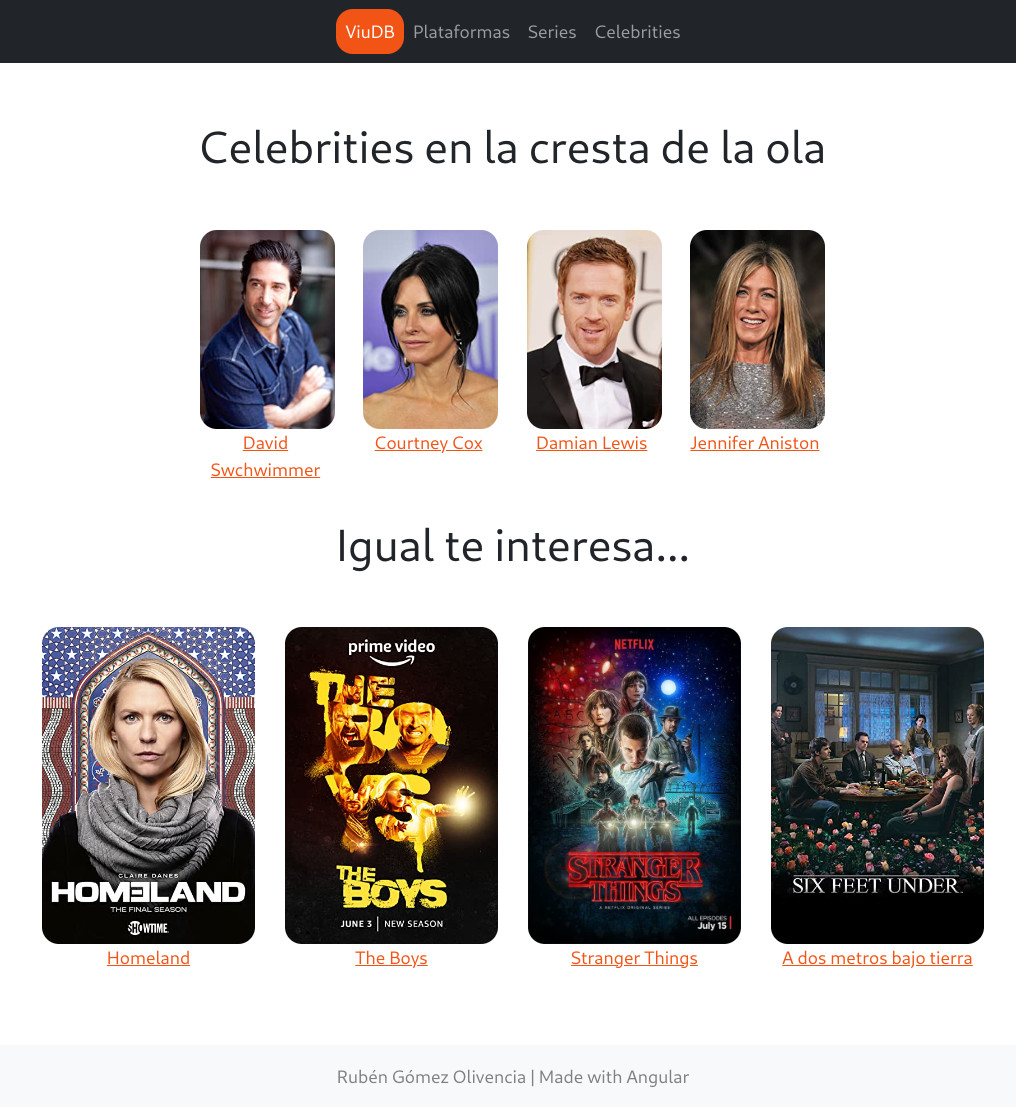
\includegraphics[frame,width=0.6\linewidth]{img/inicio.png}
\end{center}

No sólo vamos a poder visualizar la información de las distintas series, si no que también podremos visualizar el trailer de las mismas, y de esta manera saber si nos puede interesar empezar a ver la serie.

\chapter{Desarrollo realizado}
Tal como se ha indicado previamente, para realizar este proyecto se ha utilizado \href{https://angular.io/}{Angular} como \textit{framework} de desarrollo, por lo que vamos a diferenciar distintos aspectos utilizados con él.

\section{Uso de componentes}
Una de las características de Angular es la creación de componentes, para de esta manera poder separar la aplicación en distintos apartados que se pueden programar de manera separada, y tener su estilo propio.

Por ello, antes de comenzar con el desarrollo, se pensó cómo iba a ser el aspecto final de la aplicación y en cuántos componentes se iba a separar, así como la manera de poder reutilizarlos.

Si miramos, por ejemplo, la web de detalle de una plataforma, podemos diferenciar los siguientes componentes, que han sido diferenciados con distintos colores:

\vspace{-1em}
\begin{center}
    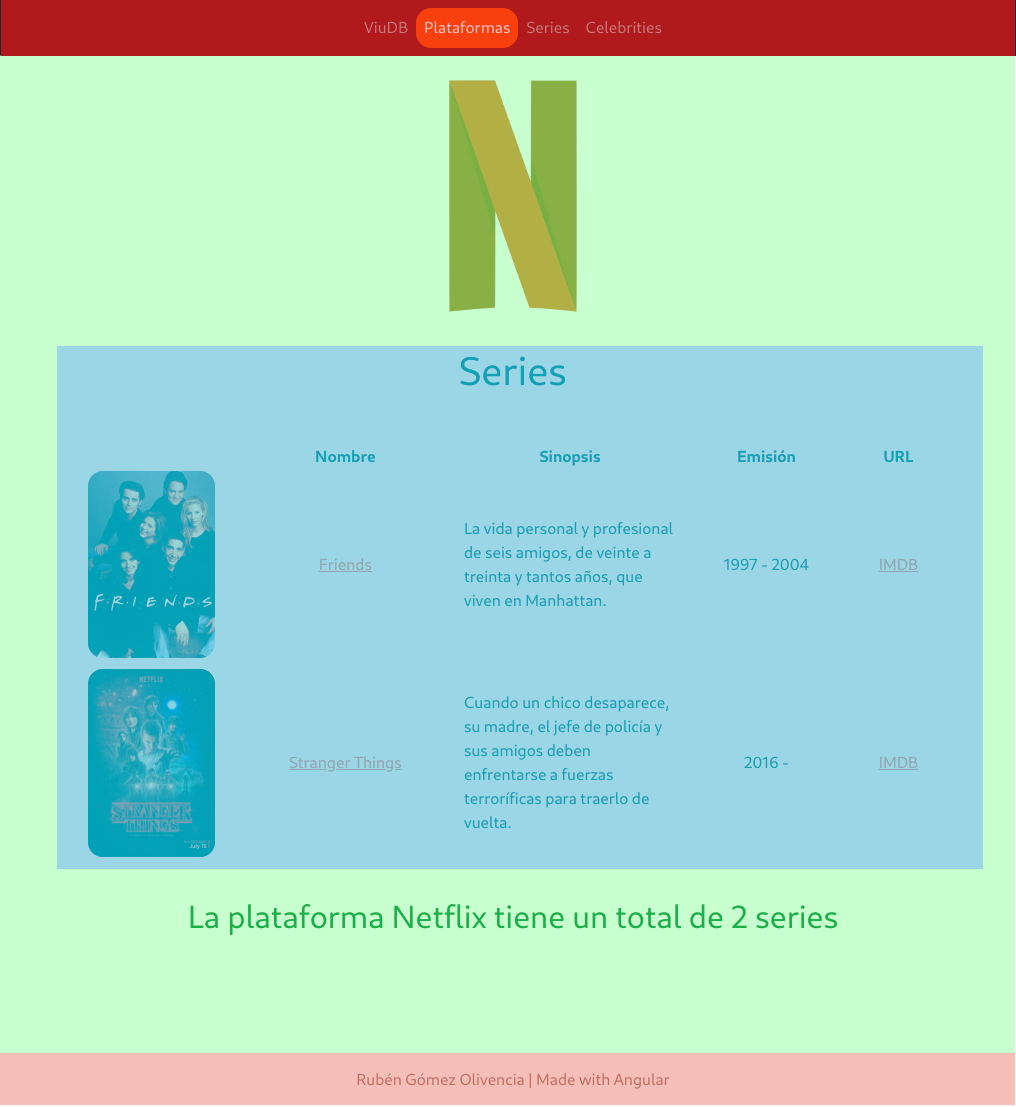
\includegraphics[frame,width=0.6\linewidth]{img/componentes.png}
\end{center}

\begin{itemize}
    \item \textbf{Cabecera}: La cabecera, o \textit{\textbf{navbar}}, nos permite ir a cualquiera de las secciones principales de la aplicación desde cualquier lugar de la misma, ya que siempre es visible. Nos indicará en qué sección estamos cambiando el color de la misma.

    \item \textbf{Sección principal}: Es donde se va a visualizar el contenido dinámico de la aplicación. Esta sección puede contener a su vez otros componentes “hijos”.

    En este caso, se está utilizando el componente que muestra una plataforma, que a su vez llama al componente de series para mostrar únicamente las series que pertenecen a esta plataforma (colores verde y azul).

    \item \textbf{Pie de página}: También conocido como \textit{footer}, al igual que la cabecera, se muestra siempre. En este caso muestra el autor de la aplicación, pero en aplicaciones más complejas podría contener también enlaces a distintos apartados de la web, web de contacto, mapa de localización...
\end{itemize}

\section{Rutas y navegación}
Como la aplicación cuenta con distintas secciones principales, es conveniente que estas sean accesibles a través de distintas URLs para poder ser enlazadas. Es aquí donde entra en juego el \textbf{\textit{routing}}.

\begin{mycode}{Parte del fichero \textbf{app.routing.ts} }{typescript}{}
const appRoutes: Routes = [
  {path: '', component: InicioComponent},
  {path: 'plataformas', component: PlataformasComponent},
  {path: 'plataformas/:id', component: PlataformasShowComponent},
  {path: 'series', component: SeriesComponent},
  {path: 'series/:id', component: SeriesShowComponent},
  {path: 'celebrities', component: CelebritiesComponent},
  {path: 'celebrities/:id', component: CelebritiesShowComponent},
  {path: '**', component: ErrorComponent},
];
\end{mycode}

Tal como se puede ver en el código, se han creado ocho rutas distintas que harán uso de distintos componentes dependiendo de cuál sea la ruta seleccionada.

La selección del componente a mostrar se realiza gracias a la configuración mostrada previamente, la URL a la que accedamos y el apartado \inlineconsole{<router-outlet></router-outlet>} dentro del fichero \configfile{app.component.html}.

Es interesante destacar la última línea de la configuración, ya que en caso de que la URL no coincida con ninguna de las anteriores, lo que hará será visualizar el componente \textbf{ErrorComponent}, en el cual se ha indicado el típico mensaje “404”.


\section{Paso de parámetros entre componentes}

Tal como se ha indicado previamente, la aplicación se ha realizado teniendo en cuenta las ventajas que nos permite el uso de componentes, y pensando en todo momento para que puedan ser reutilizados.

Esta reutilización se consigue pudiendo llamar desde un componente a otro y haciendo uso del paso de parámetros. De esta manera, podemos variar el comportamiento, y el aspecto, del componente dependiendo de cuál es el origen desde el que se le llama.

El ejemplo más claro es el componente \textbf{”series”}, que se encarga de obtener las series, y dependiendo del lugar desde donde se le llama,  visualizarlas de manera distinta.

Este componente se reutiliza (y por tanto, recibe parámetros), desde tres sitios distintos:
\begin{itemize}
    \item \textbf{Página de inicio}: Se llama al componente con el valor “-1”, para de esta manera saber que se está llamando desde la página de inicio, y por tanto que visualice cuatro series de manera aleatoria y con aspecto horizontal.

    \begin{center}
        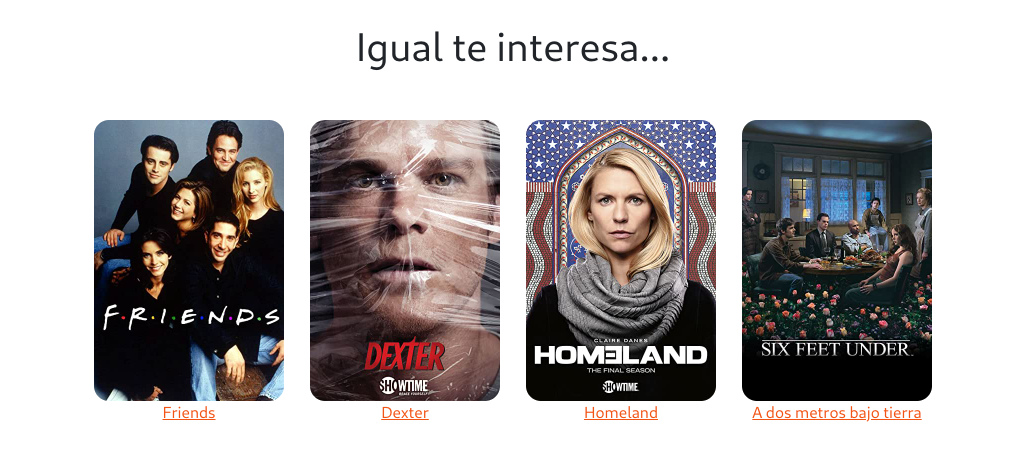
\includegraphics[frame,width=0.7\linewidth]{img/series-1.png}
    \end{center}

    \item \textbf{Sección “Series”}: Cuando se llama desde el menú principal, no se llama desde otro componente, por lo que el parámetro está inicializado a cero.

    En este caso nos visualiza todas las series con toda la información en formato tabla. Cada fila es una serie y cada columna tiene distinta información acerca de la misma.
    \vspace{-0.2em}
    \begin{center}
        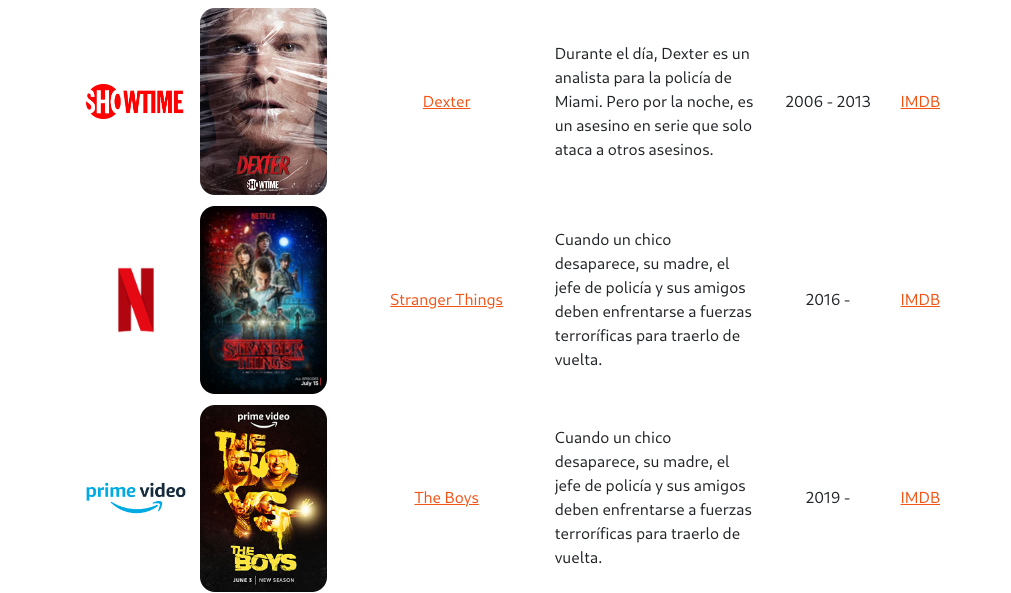
\includegraphics[frame,width=0.7\linewidth]{img/series-2.png}
    \end{center}

    \item \textbf{Información de una plataforma}: Al ir al detalle de una plataforma nos muestra todas las series de esa plataforma. Se llama al componente Series pasando como parámetro el identificador de la plataforma, para así sólo visualizar sus series.

    En este caso, el aspecto visual es similar al caso anterior, pero no se muestra la primera columna, que es la plataforma en el caso anterior, ya que quedaría redundante.

    \vspace{-0.2em}
    \begin{center}
        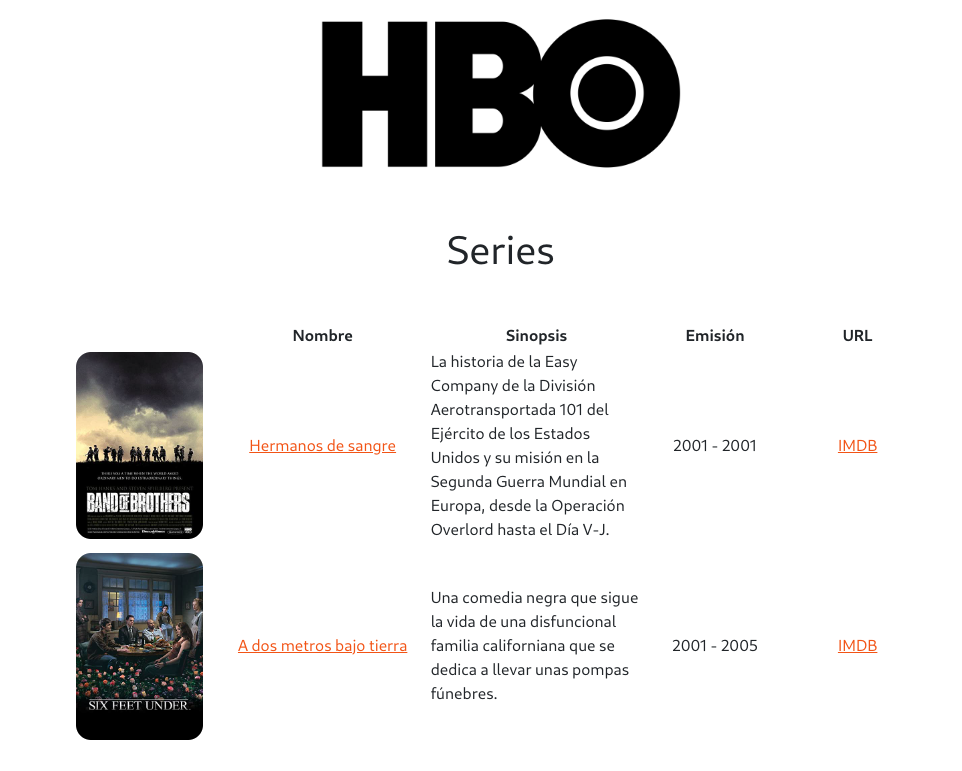
\includegraphics[frame,width=0.7\linewidth]{img/series-3.png}
    \end{center}
\end{itemize}


\subsection{Información desde el componente hijo al padre}
Hasta ahora se ha visto cómo un componente “hijo” recibe parámetros desde el componente “padre” que le llama. Pero la información también puede fluir en sentido contrario.

Esto se ha utilizado para mostrar el número de series que tiene una plataforma. El componente hijo (“Series”) es quien procesa la información, por lo que al terminar de mostrarla y visualizarla, le envía al padre el número total de series que tiene la plataforma.

\begin{mycode}{Llamada al componente “\textbf{series}” desde “\textbf{plataformas-show}”}{html+ng2}{ {\small }}
<div>
    <app-series [plataforma_id]="plataforma.id"
                (series_count)="series_count=$event">
    </app-series>
</div>

<h2>La plataforma {{plataforma.nombre}}  tiene un total de {{series_count}}
    {{series_count>1?"series":"serie"}}</h2>
\end{mycode}

En el código expuesto, se puede ver cómo se llama al componente “series” pasando el parámetro “plataforma\_id” para que sepa qué series tiene que mostrar. A su vez, del componente recibiremos información a través de un evento que guardaremos en la variable \inlineconsole{series_count} para después visualizarla en una etiqueta “h2”.


\section{Reproducción de vídeo}

Como característica multimedia, la aplicación tiene un botón para poder realizar la reproducción del trailer de la serie cuya información se está visualizando en ese momento.

Al hacer click en el botón se cargará un “modal” con el reproductor multimedia basado en \textbf{HTML5} con el que reproducir el vídeo.

Una vez más, se ha hecho uso de un componente separado para esta característica. Sólo se llama cuando se está visualizando la información completa de una serie, y recibe como parámetro parte la información de la serie para cargar la URL del trailer.


\begin{center}
    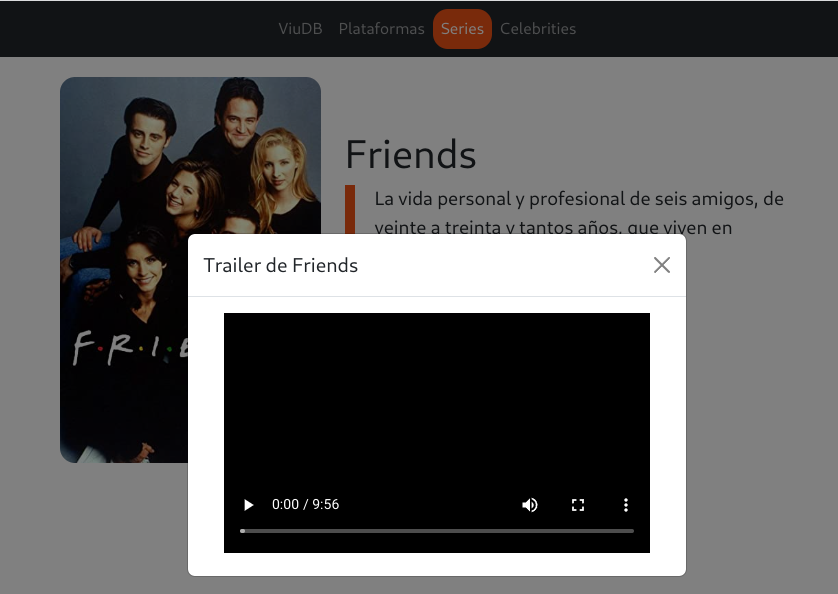
\includegraphics[frame,width=0.7\linewidth]{img/video.png}
\end{center}

\section{Otras características}
Aunque no eran requisitos del proyecto, se ha tenido especial cuidado en el diseño de la aplicación para evitar errores y tenerla preparada para el futuro.

\subsection{Control de identificadores no existentes}
Para evitar que la aplicación pueda dar información incorrecta o errores, se ha tenido especial cuidado en aquellas rutas en las que se recibe un parámetro a través de la URL.

En todos los componentes en los que se recibe un identificador se comprueba que este exista, y en caso de no ser así, la aplicación muestra un error controlado.

Así mismo, y tal como se ha dicho previamente, se cuenta con un componente que se visualiza cuando la ruta no coincide con ninguna otra válida. A continuación se pueden ver ambos errores controlados.

{
    \hfill
    \begin{minipage}{0.4\linewidth}
        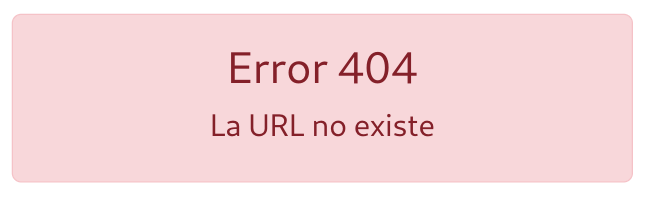
\includegraphics[width=\linewidth]{img/error1.png}
    \end{minipage}
    \hfill
    \begin{minipage}{0.4\linewidth}
        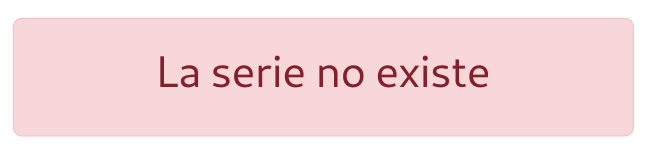
\includegraphics[width=\linewidth]{img/error2.png}
    \end{minipage}
    \hfill
}


\subsection{Datos en formato JSON}
Aunque el contenido de la información es estático (no se hace uso de peticiones a servicios externos), la información está contenida en unos ficheros JSON que emulan peticiones a una API externa.

Estos ficheros están dentro del directorio \configdir{src/assets/json/}, diferenciados para cada uno de los modelos utilizados para la aplicación: \textbf{celebrity, plataforma} y \textbf{serie}.


\chapter{Dificultades del proyecto}

Como todo proyecto de programación, durante el desarrollo nos podemos encontrar con ciertas dificultades que deben ser subsanadas para llegar a cumplir los requisitos planteados al comienzo del proyecto.

En este caso, al no haber realizado ningún proyecto previo con Angular, y no haber desarrollado con Typescript, ha hecho que el tiempo de desarrollo se haya incrementado ligeramente por errores de sintaxis y conceptos poco afianzados.

Afortunadamente, el desarrollo con Angular y Typescript es sencillo, existe abundante documentación, y los mensajes de error son lo suficientemente precisos como para saber en qué se está fallando mientras se desarrolla.



\chapter{Mejoras a realizar}

Ya se ha comentado que el proyecto se ha desarrollado planeando posibles futuras mejoras, y la principal sería hacer uso de llamadas a servicios externos para recuperar la información de series a mostrar.

Existen distintos servicios que se podrían utilizar:  \href{https://imdb-api.com/API}{API de IMDB}, \href{https://thetvdb.com/api-information}{API de TVdb} o \href{https://www.themoviedb.org/documentation/api}{API de TheMovieDB} por ejemplo. Dado que actualmente se hace uso de los ficheros JSON nombrados previamente, realizar el cambio no supondría demasiado esfuerzo, y lo único que habría que hacer es conocer los campos de la información recibida.


\chapter{Conclusiones}

A la hora de afrontar un proyecto nuevo utilizando un lenguaje de programación, o \textit{framework}, no visto hasta el momento, es importante tratar de tener una mente abierta y evitar realizar comparaciones con lo ya conocido.

Es beneficioso aplicar los conocimientos previos y la experiencia sobre un desarrollo nuevo, pero al hacerlo sobre un lenguaje o un \textit{framework} puede suponer realizar comparaciones injustas.

En este caso, al ser la primera vez que el desarrollador usa un framework completo para el \textit{front-end} se ha evitado dicha comparación, y ha dado lugar a una grata experiencia y la adquisición de nuevos conocimientos que serán utilizados en el futuro para otros proyectos.

\end{document}
